\chapter{Υλικό και Τεχνολογία \te{AoA}}
Καθώς στην συγκεκριμένη εργασία εστιάσαμε μόνο στον εντοπισμό με την χρήση \te{AoA}, στο συγκεκριμένο κεφαάλαιο θα
εξετάσουμε τις διάφορες λύσεις που είναι διαθέσιμες σε επίπεδο υλικού.

\section{\te{XPLR-AOA-1}}
Η πρώτη συσκευή που θα εξετάσουμε είναι η \te{XPLR-AOA-1}. Όλα τα προϊόντα που προσφέρουν υπολογισμούς
\te{AoA} περιλαμβάνουν τουλάχιστον τα εξής: Ένα σετ απο \te{anchors} και μια συσκευή που ονομάζεται \te{tag}. Τα \te{anchors}
ουσιαστικά είναι συστχοιχίες κεραιών, που υπολογίζουν την γωνία \te{AoA} ενός πομπού, ενώ το \te{tag} είναι η συσκευή πομπού
που προσομοιώνει έναν χρήστη. \\~\\
Η συσκευή \te{XPLR-AOA-1} εκτός απο την γωνία στο επίπεδο (\te{azimuth}), υπολογίζει και την γωνία στο ύψος (\te{altidute}),
για αυτόν τον λόγο στην πραγματικότητα έχει δυο συστοιχίες κεραιών. Η πρώτη αντιστοιχεί στο επίπεδο και είναι
διατεταγμένη οριζόντια, ενώ η δεύτερη αντιστοιχεί στο ύψος και είναι διατεταγμένη κάθετα.
\begin{figure}[h]
\centering
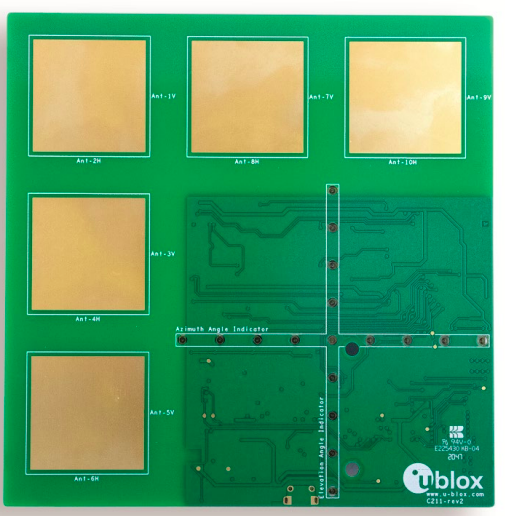
\includegraphics[width=8cm]{pictures/xplr-anchor.png}
\caption{\te{XPLR Anchor}\cite{xplr-guide}}
\end{figure}
\begin{figure}[h]
\centering
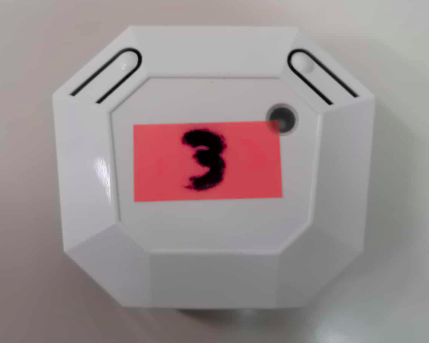
\includegraphics[width=4cm]{pictures/xplr-tag.png}
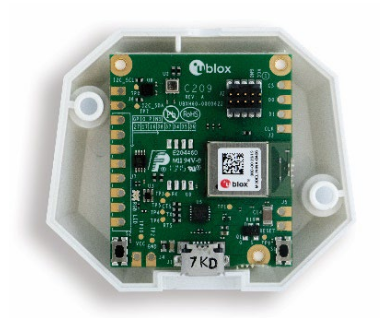
\includegraphics[width=4cm]{pictures/xplr-tag-open.png}
\caption{\te{XPLR Tag}\cite{xplr-guide}}
\end{figure}
Το \te{tag} και τα \te{anchors} του πακέτου \te{XPLR} βασίζονται στην τεχνολογία \te{Bluetooth 5.1}, τα \te{anchors} χρησιμοποιούν εσωτερικά τον \te{NINA-B411 tranceiver} ενώ το \te{tag} χρησιμοποιεί τον \te{NINA-B406}
